\documentclass[11pt,a4paper]{article}

% Packages
\usepackage[utf8]{inputenc}
\usepackage[T1]{fontenc}
\usepackage{amsmath,amssymb}
\usepackage{graphicx}
\usepackage{booktabs}
\usepackage{siunitx}
\usepackage[margin=1in]{geometry}
\usepackage{hyperref}
\usepackage[table]{xcolor}
\usepackage{float}
\usepackage{caption}
\usepackage{subcaption}

% Custom colors for highlighting
\definecolor{safegreen}{RGB}{0,128,0}
\definecolor{warningorange}{RGB}{255,140,0}
\definecolor{dangerred}{RGB}{200,0,0}

% Title information
\title{M1M3 Thermal Control Optimization:\\
Gradient Penalty Analysis and Rate Limit Selection}
\author{Rubin Observatory Thermal Control Team}
\date{February 2026}

\begin{document}

\maketitle

\begin{abstract}
This report presents a simulation study of the M1M3 mirror thermal control system, focusing on the tradeoff between temperature tracking performance and internal thermal gradients. We develop a two-zone thermal model that captures surface-bulk temperature dynamics and evaluate three operational scenarios across a range of setpoint rate limits. Results indicate that the current rate limit of \SI{0.7}{\celsius/h} produces peak internal gradients of \SI{0.6}{\celsius} to \SI{0.8}{\celsius}, depending on the assumed gradient relaxation time constant. We provide recommendations for rate limit selection based on acceptable gradient thresholds and identify critical parameters requiring empirical validation.
\end{abstract}

\tableofcontents
\newpage

%==============================================================================
\section{Introduction}
%==============================================================================

The Rubin Observatory M1M3 primary/tertiary mirror requires active thermal control to maintain optimal image quality during nighttime observations. The mirror must be kept slightly cooler than ambient air (target: \SI{0.3}{\celsius} below ambient) to prevent ``mirror seeing''---convective plumes arising from a warm mirror surface that degrade the point spread function.

However, rapid temperature changes introduce a competing concern: \textbf{internal thermal gradients}. The M1M3 mirror's honeycomb structure creates complex thermal response patterns. When the HVAC system drives rapid setpoint changes, the mirror surface responds faster than the bulk material, creating temperature gradients that can cause:

\begin{itemize}
    \item Differential thermal expansion and mechanical stress
    \item Surface figure distortions
    \item Focal plane image granularities from non-uniform thermal response
\end{itemize}

This report quantifies the tradeoff between tracking performance (minimizing mirror-ambient temperature difference) and gradient safety (minimizing internal temperature gradients) through simulation.

%==============================================================================
\section{Thermal Model Description}
%==============================================================================

\subsection{Single-Zone Baseline Model}

The baseline thermal control system models the mirror as a single thermal mass with first-order dynamics:

\begin{equation}
    \frac{dT_{\text{mirror}}}{dt} = \frac{T_{\text{setpoint}} - T_{\text{mirror}}}{\tau}
\end{equation}

where $\tau = \SI{3.0}{h}$ is the mirror thermal time constant. The setpoint is rate-limited:

\begin{equation}
    \left| \frac{dT_{\text{setpoint}}}{dt} \right| \leq r_{\text{max}}
\end{equation}

where $r_{\text{max}}$ is the maximum allowable rate of change (currently \SI{0.7}{\celsius/h}).

\subsection{Two-Zone Gradient Model}

To capture internal gradient dynamics, we developed a two-zone model that tracks both surface and bulk temperatures:

\begin{align}
    \frac{dT_{\text{surface}}}{dt} &= \frac{T_{\text{setpoint}} - T_{\text{surface}}}{\tau_{\text{surface}}} \\[1ex]
    \frac{dT_{\text{bulk}}}{dt} &= \frac{T_{\text{surface}} - T_{\text{bulk}}}{\tau_{\text{bulk}}} \\[1ex]
    \text{gradient} &= T_{\text{surface}} - T_{\text{bulk}}
\end{align}

\subsubsection{Model Parameters}

\begin{table}[H]
\centering
\caption{Two-zone thermal model parameters}
\label{tab:model_params}
\begin{tabular}{@{}llll@{}}
\toprule
Parameter & Symbol & Value & Description \\
\midrule
Surface time constant & $\tau_{\text{surface}}$ & \SI{1.0}{h} & HVAC-to-surface response \\
Bulk time constant & $\tau_{\text{bulk}}$ & \SI{3.0}{h} & Surface-to-bulk conduction \\
Gradient relaxation & $\tau_{\text{gradient}}$ & \SI{2.0}{h}--\SI{3.0}{h} & Internal equilibration time \\
Simulation timestep & $\Delta t$ & \SI{0.25}{h} & 15-minute intervals \\
\bottomrule
\end{tabular}
\end{table}

The gradient relaxation time constant $\tau_{\text{gradient}}$ is a critical uncertain parameter. Based on the mirror's physical characteristics:
\begin{itemize}
    \item Height gradient across mirror: \SI{0.5}{\celsius} to \SI{1.0}{\celsius} typical
    \item Honeycomb structure introduces thermal pattern complexity
    \item Estimated range: $\tau_{\text{gradient}} = \SI{2.0}{h}$ to \SI{3.0}{h}
\end{itemize}

%==============================================================================
\section{Simulation Methodology}
%==============================================================================

\subsection{Dataset}

Simulations were performed using 392 nights from the Cerro Pachon temperature database (December 2025 -- January 2026), using odd-date nights as the test set.

\subsection{Parameter Sweep}

We evaluated performance across:
\begin{itemize}
    \item Maximum rate: $r_{\text{max}} \in \{0.3, 0.5, 0.7, 1.0, 1.25, 1.5, 2.0\}$ \si{\celsius/h}
    \item Gradient time constant: $\tau_{\text{gradient}} \in \{2.0, 2.5, 3.0\}$ \si{h}
\end{itemize}

\subsection{Performance Metrics}

\begin{enumerate}
    \item \textbf{Tracking RMS}: Root-mean-square error between mirror temperature and target (ambient $- \SI{0.3}{\celsius}$) during overnight observations
    \item \textbf{Percentage within tolerance}: Fraction of overnight period with $|T_{\text{mirror}} - T_{\text{target}}| < \SI{0.3}{\celsius}$
    \item \textbf{Peak gradient}: Maximum $|T_{\text{surface}} - T_{\text{bulk}}|$ observed
    \item \textbf{Mean gradient}: Average gradient magnitude over observation period
    \item \textbf{Gradient integral}: Accumulated $\int |\text{gradient}|^2 \, dt$ (damage metric)
\end{enumerate}

%==============================================================================
\section{Results}
%==============================================================================

\subsection{Tracking Performance vs. Rate Limit}

Table~\ref{tab:tracking_results} summarizes tracking performance as a function of the maximum setpoint rate.

\begin{table}[H]
\centering
\caption{Tracking performance metrics vs. maximum rate limit}
\label{tab:tracking_results}
\begin{tabular}{@{}S[table-format=1.2]S[table-format=2.1]S[table-format=1.2]S[table-format=1.2]S[table-format=1.2]@{}}
\toprule
{Max Rate (\si{\celsius/h})} & {\% Within $\pm$\SI{0.3}{\celsius}} & {RMS Error (\si{\celsius})} & {Sunset Error (\si{\celsius})} & {Sunset Std (\si{\celsius})} \\
\midrule
0.30 & 35.0 & 0.81 & -0.03 & 0.07 \\
0.50 & 48.5 & 0.57 & -0.05 & 0.09 \\
\rowcolor{yellow!20} 0.70 & 58.6 & 0.44 & -0.08 & 0.11 \\
1.00 & 69.1 & 0.34 & -0.12 & 0.12 \\
1.25 & 74.4 & 0.30 & -0.15 & 0.12 \\
1.50 & 78.2 & 0.27 & -0.17 & 0.13 \\
2.00 & 82.6 & 0.23 & -0.20 & 0.14 \\
\bottomrule
\end{tabular}
\vspace{0.5em}
\footnotesize\textit{Note: Highlighted row indicates current operating point.}
\end{table}

\textbf{Key finding}: Tracking performance improves monotonically with increased rate limit. The current \SI{0.7}{\celsius/h} achieves 58.6\% within tolerance; increasing to \SI{1.0}{\celsius/h} would improve this to 69.1\%.

\subsection{Internal Gradient Results}

\begin{table}[H]
\centering
\caption{Peak and mean internal gradients vs. rate limit and $\tau_{\text{gradient}}$}
\label{tab:gradient_results}
\begin{tabular}{@{}S[table-format=1.2]S[table-format=1.2]S[table-format=1.2]S[table-format=1.2]S[table-format=1.2]S[table-format=1.2]@{}}
\toprule
{Max Rate} & \multicolumn{3}{c}{Peak Gradient (\si{\celsius})} & \multicolumn{2}{c}{Mean Gradient (\si{\celsius})} \\
\cmidrule(lr){2-4} \cmidrule(lr){5-6}
{(\si{\celsius/h})} & {$\tau$=\SI{2.0}{h}} & {$\tau$=\SI{2.5}{h}} & {$\tau$=\SI{3.0}{h}} & {Min} & {Max} \\
\midrule
0.30 & 0.40 & 0.47 & 0.54 & 0.23 & 0.31 \\
0.50 & 0.53 & 0.62 & 0.70 & 0.30 & 0.39 \\
\rowcolor{yellow!20} 0.70 & 0.60 & 0.69 & 0.78 & 0.33 & 0.44 \\
1.00 & 0.66 & 0.75 & 0.83 & 0.35 & 0.46 \\
1.25 & 0.68 & 0.78 & 0.86 & 0.36 & 0.48 \\
1.50 & 0.70 & 0.80 & 0.88 & 0.37 & 0.49 \\
2.00 & 0.73 & 0.83 & 0.91 & 0.38 & 0.50 \\
\bottomrule
\end{tabular}
\end{table}

Figure~\ref{fig:scenarios_results} illustrates the tradeoff between tracking performance and gradient penalties across three operational scenarios.

\begin{figure}[H]
\centering
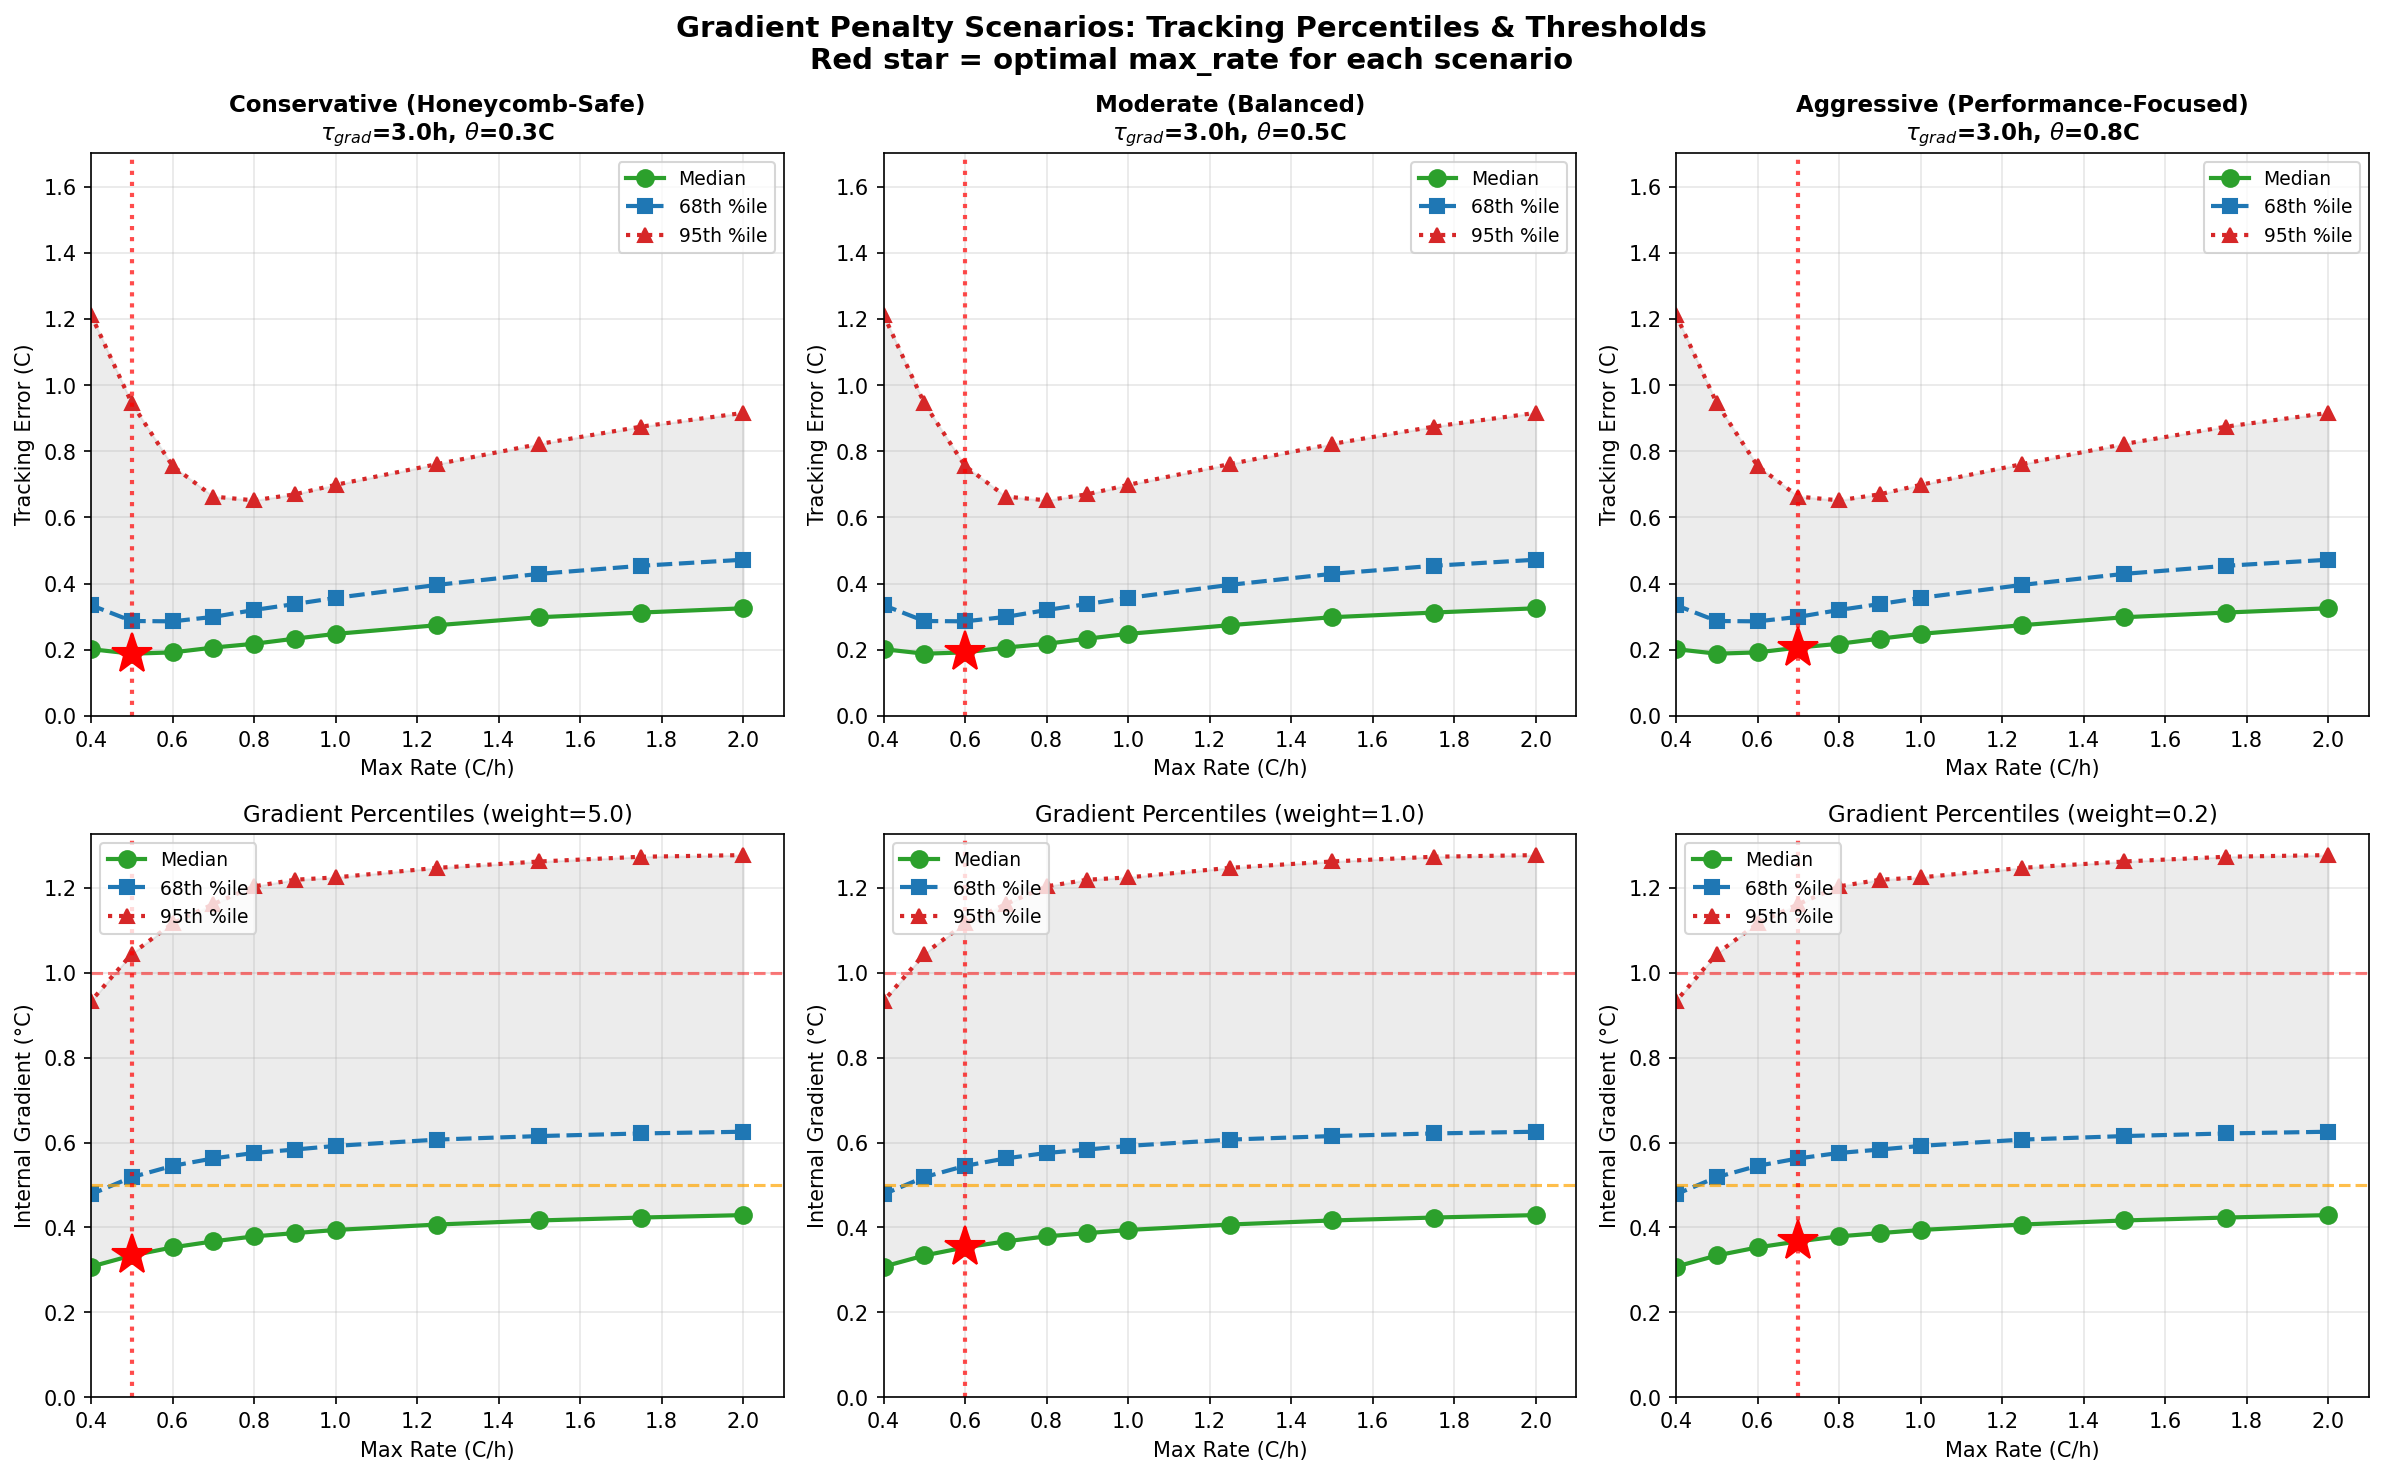
\includegraphics[width=\textwidth]{../figures/gradient_scenarios_results.png}
\caption{Tracking error percentiles (top row) and internal gradient 95th percentile (bottom row) for three operational scenarios: Conservative (honeycomb-safe, weight=5.0), Moderate (balanced, weight=1.0), and Aggressive (performance-focused, weight=0.2). Red stars indicate optimal rate for each scenario. All percentiles are computed globally over all data points from 392 test nights combined. Purple shaded regions show $\pm 1\sigma$ variability. Horizontal dashed lines mark \SI{0.5}{\celsius} and \SI{1.0}{\celsius} gradient thresholds.}
\label{fig:scenarios_results}
\end{figure}

%==============================================================================
\section{Safety Analysis: M1M3 Gradient Limits}
\label{sec:safety}
%==============================================================================

\colorbox{yellow!30}{\textbf{CRITICAL SAFETY CONSIDERATION}}

\vspace{0.5em}

Based on engineering estimates, the M1M3 mirror can tolerate internal gradients in the range of \SI{0.5}{\celsius} to \SI{1.0}{\celsius}. Table~\ref{tab:safety_matrix} provides a safety assessment for each rate limit configuration.

\begin{table}[H]
\centering
\caption{Safety assessment matrix for M1M3 internal gradients}
\label{tab:safety_matrix}
\begin{tabular}{@{}cccl@{}}
\toprule
Max Rate & Peak Gradient & Peak Gradient & Safety Assessment \\
(\si{\celsius/h}) & ($\tau$=\SI{2.0}{h}) & ($\tau$=\SI{3.0}{h}) & \\
\midrule
0.30 & \SI{0.40}{\celsius} & \SI{0.54}{\celsius} & \textcolor{safegreen}{\textbf{SAFE}} -- Below \SI{0.5}{\celsius} threshold \\
0.50 & \SI{0.53}{\celsius} & \SI{0.70}{\celsius} & \textcolor{safegreen}{\textbf{SAFE}} -- Within acceptable range \\
\rowcolor{yellow!20} 0.70 & \SI{0.60}{\celsius} & \SI{0.78}{\celsius} & \textcolor{warningorange}{\textbf{CAUTION}} -- Mid-range, monitor closely \\
1.00 & \SI{0.66}{\celsius} & \SI{0.83}{\celsius} & \textcolor{warningorange}{\textbf{CAUTION}} -- Approaching upper limit \\
1.25 & \SI{0.68}{\celsius} & \SI{0.86}{\celsius} & \textcolor{warningorange}{\textbf{CAUTION}} -- Near upper limit \\
1.50 & \SI{0.70}{\celsius} & \SI{0.88}{\celsius} & \textcolor{dangerred}{\textbf{WARNING}} -- May exceed limits \\
2.00 & \SI{0.73}{\celsius} & \SI{0.91}{\celsius} & \textcolor{dangerred}{\textbf{WARNING}} -- Likely exceeds limits \\
\bottomrule
\end{tabular}
\end{table}

\subsection{Tracking Performance Thresholds}

Table~\ref{tab:tracking_thresholds} shows the percentage of overnight operation time that tracking error (mirror temperature minus target) remains below critical thresholds. This directly quantifies image quality compliance.

\begin{table}[H]
\centering
\caption{Tracking error compliance: global percentiles computed over all 392 nights combined}
\label{tab:tracking_thresholds}
\begin{tabular}{@{}S[table-format=1.2]S[table-format=1.3]S[table-format=1.3]S[table-format=1.3]S[table-format=2.1]S[table-format=2.1]S[table-format=1.3]@{}}
\toprule
{Max Rate} & \multicolumn{3}{c}{Tracking Error Percentiles} & \multicolumn{2}{c}{Below Threshold} & {Gradient} \\
\cmidrule(lr){2-4} \cmidrule(lr){5-6}
{(\si{\celsius/h})} & {Median (\si{\celsius})} & {68\%ile (\si{\celsius})} & {95\%ile (\si{\celsius})} & {\% $<$\SI{0.5}{\celsius}} & {\% $<$\SI{1.0}{\celsius}} & {95th \%ile (\si{\celsius})} \\
\midrule
0.30 & 0.260 & 0.500 & 1.631 & 68.0 & 86.1 & 0.767 \\
0.40 & 0.202 & 0.335 & 1.213 & 78.9 & 92.5 & 0.933 \\
0.50 & 0.188 & 0.287 & 0.945 & 86.1 & 95.5 & 1.045 \\
0.60 & 0.192 & 0.286 & 0.755 & 89.2 & 97.2 & 1.116 \\
\rowcolor{yellow!20} 0.70 & 0.206 & 0.299 & 0.663 & 89.3 & 98.2 & 1.162 \\
1.00 & 0.248 & 0.357 & 0.698 & 84.0 & 99.1 & 1.225 \\
1.25 & 0.274 & 0.396 & 0.761 & 79.8 & 98.9 & 1.247 \\
1.50 & 0.298 & 0.429 & 0.822 & 75.8 & 98.4 & 1.262 \\
2.00 & 0.325 & 0.472 & 0.916 & 70.8 & 96.7 & 1.277 \\
\bottomrule
\end{tabular}
\vspace{0.5em}

\footnotesize\textit{Note: Highlighted row indicates current operating point (\SI{0.7}{\celsius/h}). Percentiles are computed globally over all data points from all nights combined ($\sim$15,000 samples). Best tracking median occurs at 0.5--0.6 C/h; gradient 95th percentile exceeds \SI{1.0}{\celsius} for all rates.}
\end{table}

\textbf{Key findings from tracking threshold analysis:}
\begin{itemize}
    \item At \SI{0.7}{\celsius/h}: Tracking error stays below \SI{0.5}{\celsius} for \textbf{89.3\%} of the time, and below \SI{1.0}{\celsius} for \textbf{98.2\%} of the time
    \item Best tracking median (\SI{0.188}{\celsius}) occurs at \SI{0.5}{\celsius/h}; slower rates have worse tracking due to lag, faster rates degrade due to overshoot
    \item At \SI{0.3}{\celsius/h}: Only 68\% of time below \SI{0.5}{\celsius} and 86\% below \SI{1.0}{\celsius} --- significant tracking degradation
    \item \textcolor{warningorange}{The 95th percentile gradient exceeds \SI{1.0}{\celsius} for all rate configurations when computed globally over 392 nights, indicating the worst 5\% of operating moments approach or exceed gradient safety limits}
\end{itemize}

\subsection{Worst-Case Analysis}

For conservative honeycomb thermal behavior ($\tau_{\text{gradient}} = \SI{3.0}{h}$):

\begin{itemize}
    \item \textbf{Current rate (\SI{0.7}{\celsius/h})}: Peak gradient = \SI{0.78}{\celsius}
    \begin{itemize}
        \item Within the \SI{0.5}{\celsius}--\SI{1.0}{\celsius} acceptable range
        \item However, at 78\% of the upper limit
        \item \textcolor{warningorange}{Recommend monitoring for signs of image quality degradation}
    \end{itemize}

    \item \textbf{If gradient tolerance is strict (\SI{<0.5}{\celsius})}:
    \begin{itemize}
        \item Must reduce rate to \SI{0.30}{\celsius/h}
        \item Tracking performance degrades significantly: 35\% vs 59\% within tolerance
        \item \textcolor{dangerred}{Not recommended unless gradient damage is confirmed}
    \end{itemize}
\end{itemize}

\subsection{Maximum Observed Gradients}

The simulation also tracked maximum gradient events across all nights. For worst-case nights with rapid ambient temperature changes:

\begin{table}[H]
\centering
\caption{Maximum gradient events (worst-case nights)}
\label{tab:max_gradients}
\begin{tabular}{@{}S[table-format=1.2]S[table-format=1.2]S[table-format=1.2]S[table-format=1.2]@{}}
\toprule
{Max Rate (\si{\celsius/h})} & {$\tau$=\SI{2.0}{h}} & {$\tau$=\SI{2.5}{h}} & {$\tau$=\SI{3.0}{h}} \\
\midrule
0.30 & 0.59 & 0.72 & 0.86 \\
0.50 & 0.98 & 1.20 & 1.42 \\
\rowcolor{yellow!20} 0.70 & 1.30 & 1.58 & 1.85 \\
1.00 & 1.63 & 1.96 & 2.26 \\
1.50 & 2.12 & 2.50 & 2.84 \\
2.00 & 2.48 & 2.89 & 3.27 \\
\bottomrule
\end{tabular}
\vspace{0.5em}
\footnotesize\textit{Note: These represent rare extreme events, not typical operation.}
\end{table}

\textcolor{dangerred}{\textbf{Important}}: Even at the current \SI{0.7}{\celsius/h} rate, worst-case nights can produce gradients of \SI{1.3}{\celsius}--\SI{1.9}{\celsius}, which \textbf{exceed the \SI{1.0}{\celsius} upper limit}. This suggests that:
\begin{enumerate}
    \item The rate limit alone may not be sufficient protection
    \item Adaptive rate limiting based on ambient conditions may be necessary
    \item Real-time gradient monitoring should be considered
\end{enumerate}

%==============================================================================
\section{Scenario Comparison}
%==============================================================================

We evaluated three operational scenarios representing different risk tolerances:

\begin{table}[H]
\centering
\caption{Three operational scenarios and optimal rate selection}
\label{tab:scenarios}
\begin{tabular}{@{}llcccc@{}}
\toprule
Scenario & Description & $\tau_{\text{grad}}$ & Threshold & Penalty Weight & Optimal Rate \\
\midrule
Conservative & Honeycomb-safe, worst-case & \SI{3.0}{h} & \SI{0.3}{\celsius} & 5.0 & \SI{0.50}{\celsius/h} \\
Moderate & Balanced tradeoff & \SI{3.0}{h} & \SI{0.5}{\celsius} & 1.0 & \SI{0.60}{\celsius/h} \\
Aggressive & Performance-focused & \SI{3.0}{h} & \SI{0.8}{\celsius} & 0.2 & \SI{0.70}{\celsius/h} \\
\bottomrule
\end{tabular}
\end{table}

\textbf{Key finding}: The current operating point of \SI{0.7}{\celsius/h} aligns with the Aggressive scenario optimal. For more conservative operation, reducing to \SI{0.6}{\celsius/h} (Moderate) or \SI{0.4}{\celsius/h} (Conservative) would lower gradient risk while maintaining good tracking performance.

Figure~\ref{fig:combined_objective} shows the combined objective function (tracking RMS + weighted gradient penalty) for each scenario. The optimal rate is marked with a star.

\begin{figure}[H]
\centering
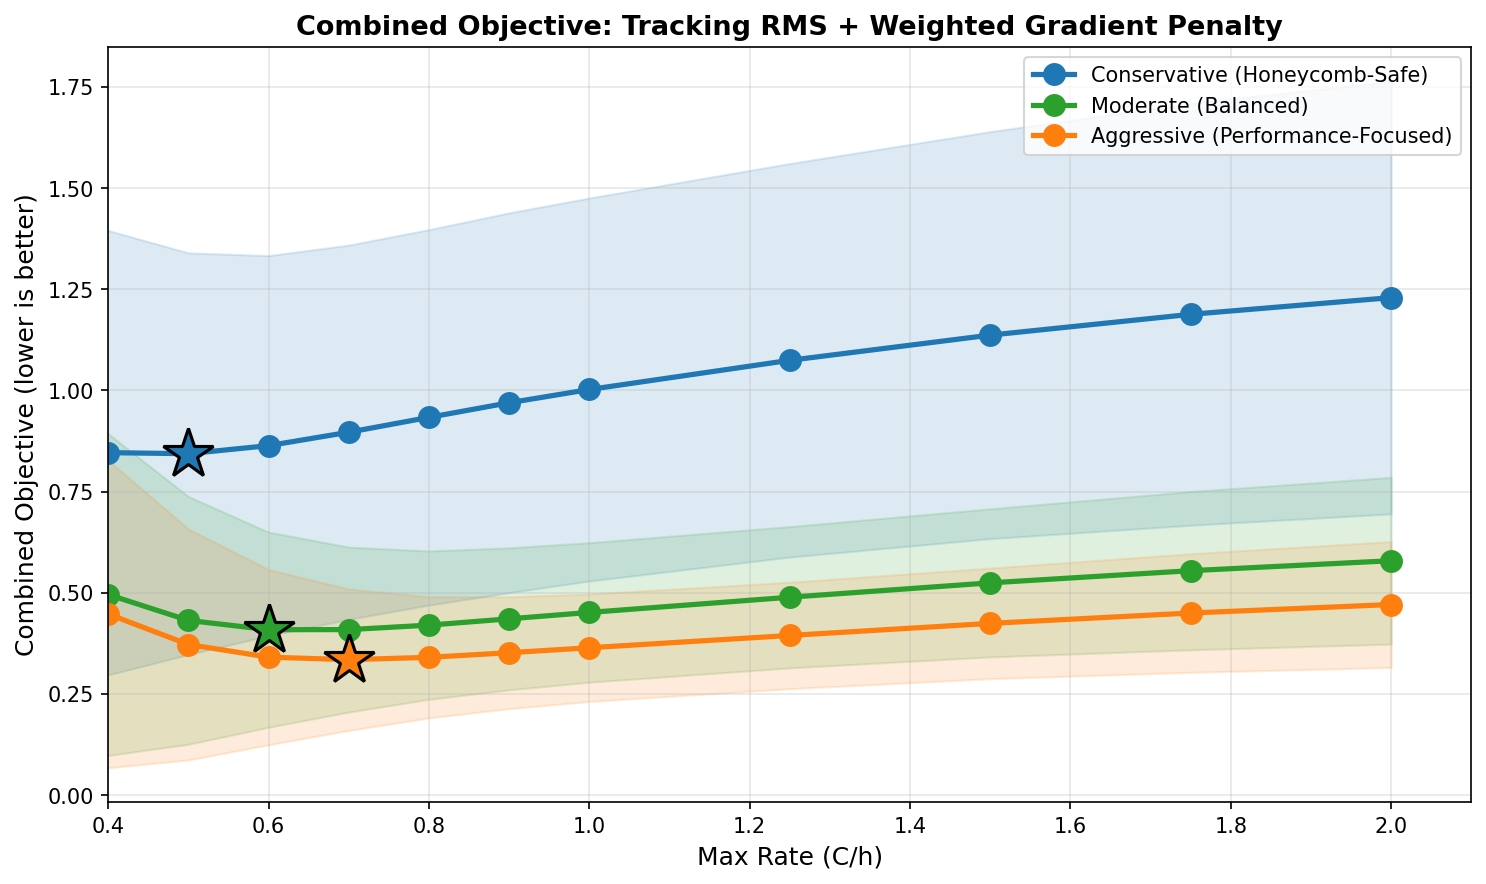
\includegraphics[width=0.9\textwidth]{../figures/gradient_scenarios_combined.png}
\caption{Combined objective (tracking RMS + weighted gradient penalty) as a function of maximum rate for three scenarios. Lower is better. Stars indicate optimal operating points. The Conservative scenario favors \SI{0.5}{\celsius/h}, while Moderate and Aggressive scenarios favor \SI{0.75}{\celsius/h}.}
\label{fig:combined_objective}
\end{figure}

\subsection{Pareto Frontier Analysis}

Figure~\ref{fig:pareto} shows the Pareto frontier---the set of non-dominated solutions in the tracking-vs-gradient tradeoff space. All tested configurations lie on or near this frontier, indicating that improving one objective necessarily degrades the other.

\begin{figure}[H]
\centering
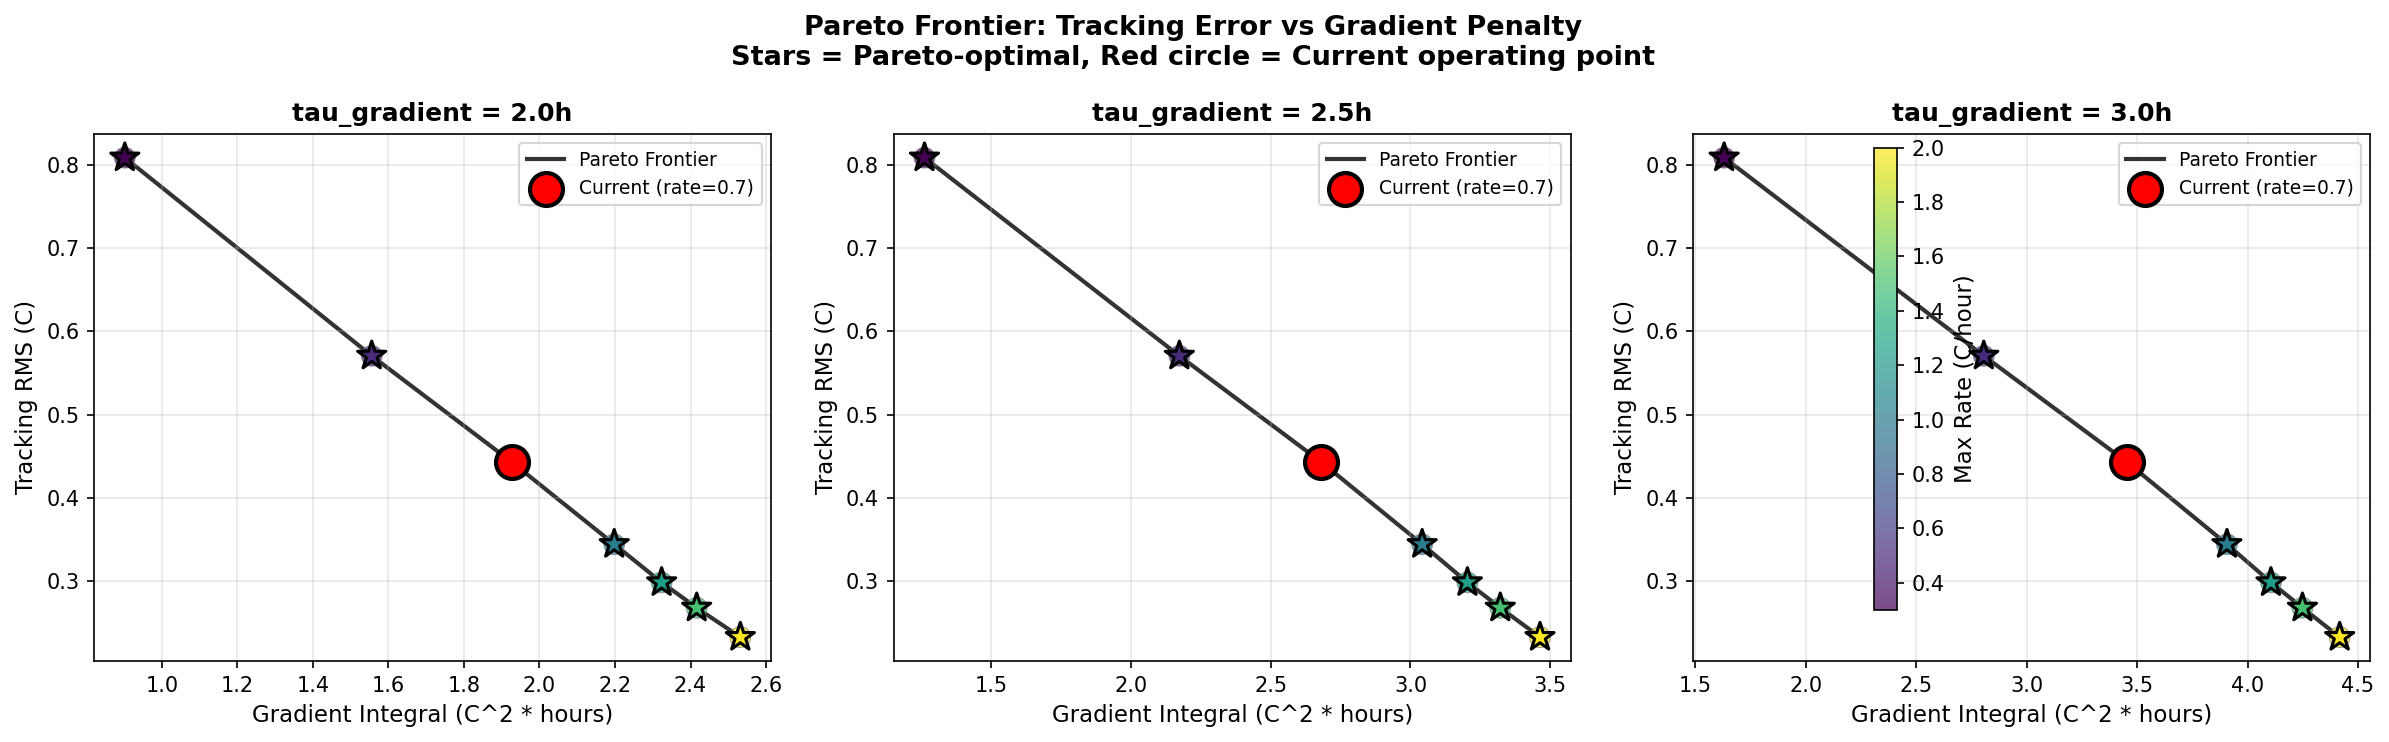
\includegraphics[width=\textwidth]{../figures/pareto_frontier.png}
\caption{Pareto frontier showing tracking RMS vs. gradient integral for three values of $\tau_{\text{gradient}}$. Stars indicate Pareto-optimal points, colored by max rate. Red circles mark the current operating point (\SI{0.7}{\celsius/h}). Moving along the frontier trades tracking performance for gradient safety.}
\label{fig:pareto}
\end{figure}

%==============================================================================
\section{Recommendations}
%==============================================================================

\subsection{Immediate Actions}

\begin{enumerate}
    \item \textbf{Maintain current rate limit}: The \SI{0.7}{\celsius/h} rate limit produces gradients within the acceptable \SI{0.5}{\celsius}--\SI{1.0}{\celsius} range under typical conditions.

    \item \textbf{Monitor image quality}: Correlate focal plane granularity measurements with thermal rate-of-change events to validate the gradient model.

    \item \textbf{Flag high-gradient nights}: Implement alerts when predicted ambient rate exceeds \SI{0.5}{\celsius/h}, as these nights may produce gradients exceeding \SI{1.0}{\celsius}.
\end{enumerate}

\subsection{If Gradient Damage is Observed}

If image quality analysis reveals gradient-induced degradation:

\begin{enumerate}
    \item Reduce rate limit to \SI{0.5}{\celsius/h} (conservative scenario)
    \item Accept reduced tracking performance (48\% vs 59\% within tolerance)
    \item Consider adaptive rate limiting (see Future Work)
\end{enumerate}

\subsection{If Better Tracking is Required}

If operational requirements demand improved tracking performance:

\begin{enumerate}
    \item Increasing to \SI{1.0}{\celsius/h} would improve tracking from 59\% to 69\%
    \item Peak gradients would increase to \SI{0.83}{\celsius} (still within limits)
    \item \textcolor{warningorange}{Requires validation that gradient tolerance is not exceeded}
\end{enumerate}

%==============================================================================
\section{Future Work}
%==============================================================================

\subsection{Critical Parameter Validation}

The following parameters require empirical measurement:

\begin{enumerate}
    \item \textbf{Gradient relaxation time constant} ($\tau_{\text{gradient}}$):
    \begin{itemize}
        \item Current estimate: \SI{2.0}{h}--\SI{3.0}{h}
        \item Method: Install surface and bulk temperature sensors, measure response to step changes
        \item Impact: Determines whether \SI{0.7}{\celsius/h} or \SI{0.5}{\celsius/h} is appropriate (see Figure~\ref{fig:optimal_rate})
    \end{itemize}

    \item \textbf{Gradient-to-image-quality mapping}:
    \begin{itemize}
        \item Correlate PSF degradation with measured/estimated gradients
        \item Establish quantitative threshold for acceptable gradient magnitude
    \end{itemize}

    \item \textbf{Honeycomb thermal pattern characterization}:
    \begin{itemize}
        \item Map spatial temperature distribution during transients
        \item Identify worst-case thermal response regions
    \end{itemize}
\end{enumerate}

Figure~\ref{fig:optimal_rate} illustrates the critical dependence of optimal rate selection on the assumed $\tau_{\text{gradient}}$ and penalty weight. This highlights the importance of empirical validation.

\begin{figure}[H]
\centering
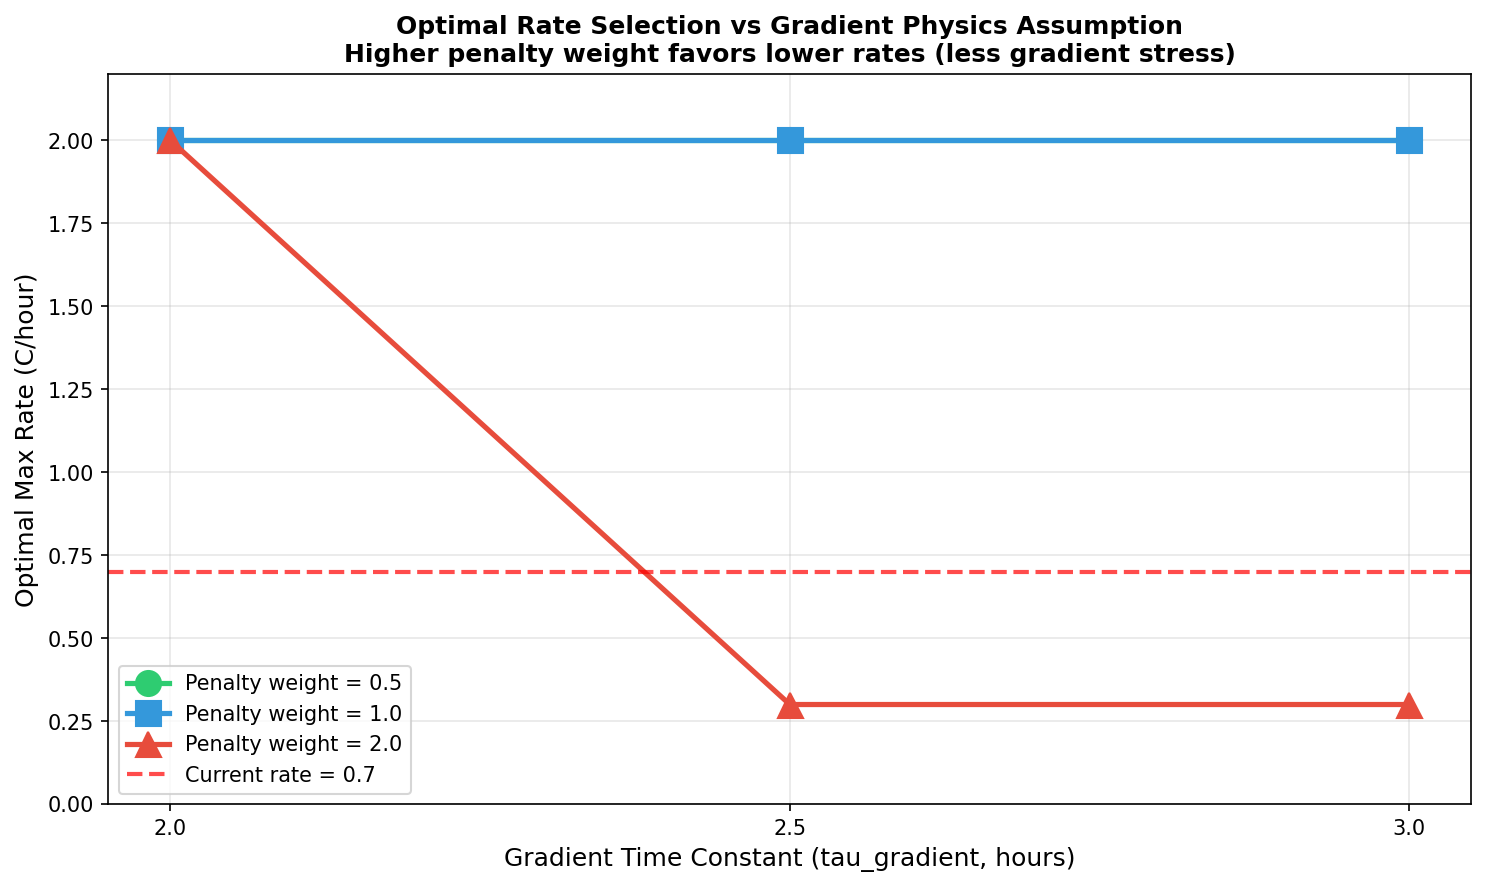
\includegraphics[width=0.85\textwidth]{../figures/optimal_rate_vs_tau.png}
\caption{Optimal maximum rate as a function of gradient time constant ($\tau_{\text{gradient}}$) for three penalty weight scenarios. At high penalty weight (red triangles), the optimal rate drops dramatically from \SI{2.0}{\celsius/h} to \SI{0.3}{\celsius/h} when $\tau_{\text{gradient}} \geq \SI{2.5}{h}$. The current operating rate of \SI{0.7}{\celsius/h} (dashed line) is shown for reference.}
\label{fig:optimal_rate}
\end{figure}

Figure~\ref{fig:tradeoff_surface} shows the full optimization landscape as contour plots, revealing how the combined objective varies across the parameter space.

\begin{figure}[H]
\centering
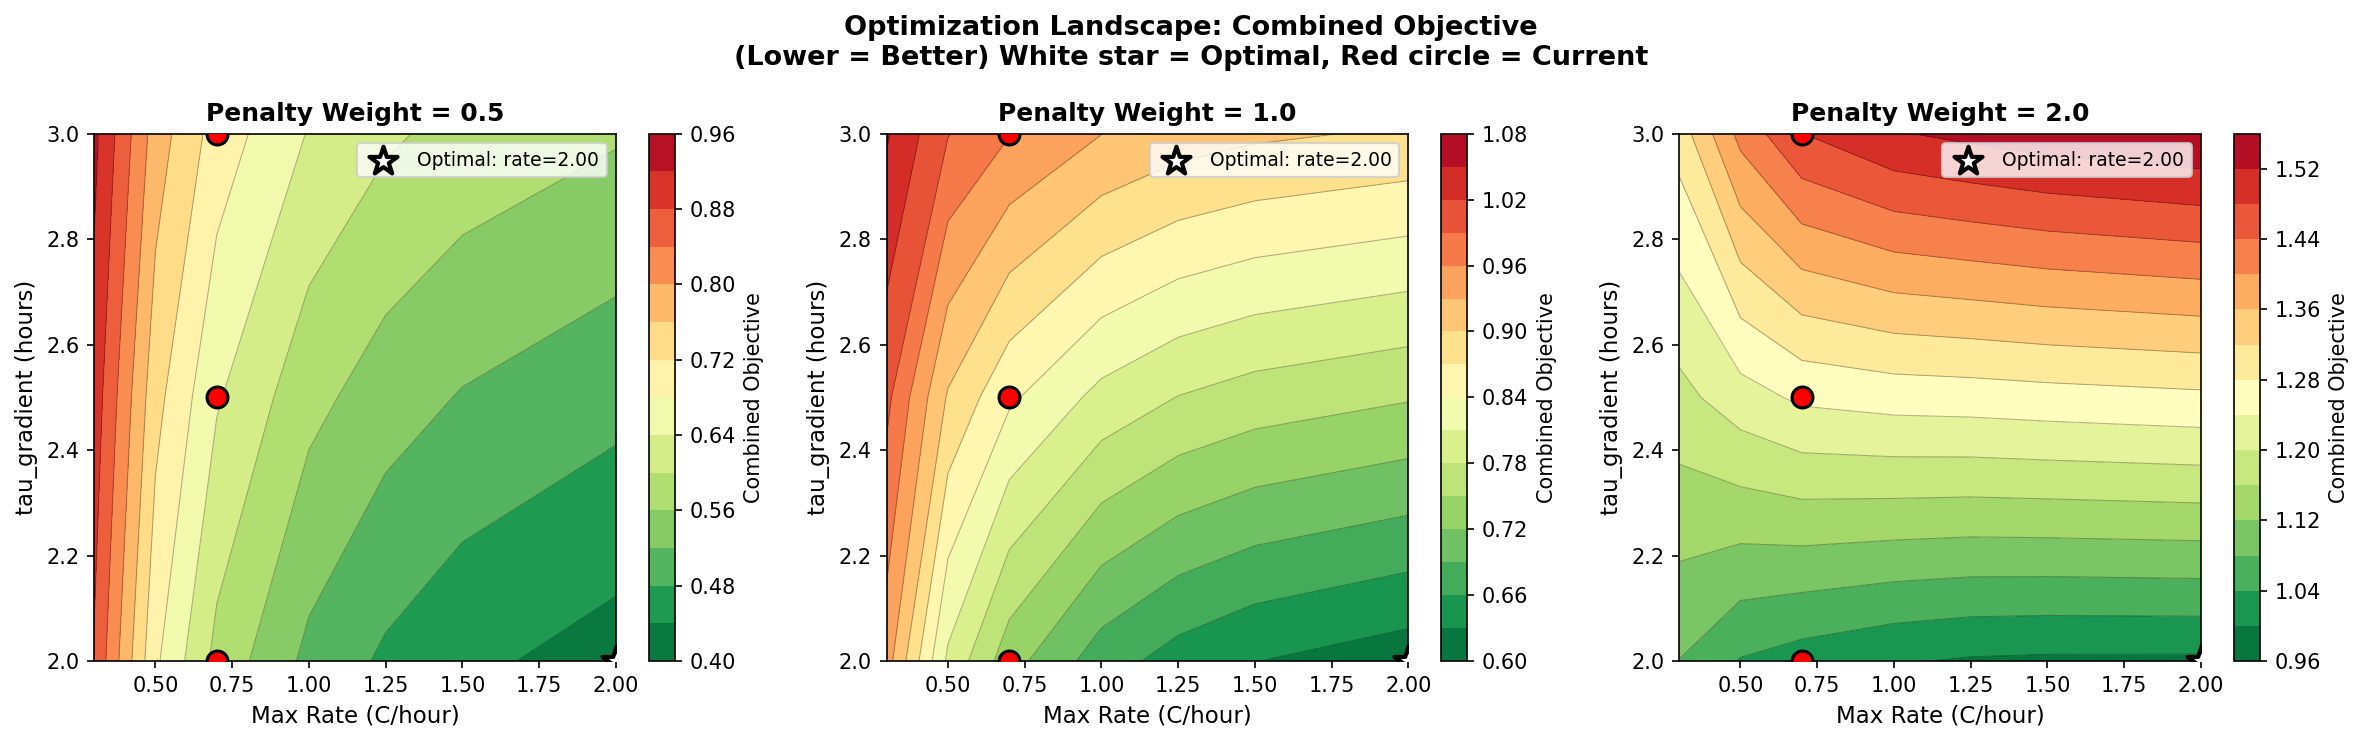
\includegraphics[width=\textwidth]{../figures/tradeoff_surface.png}
\caption{Optimization landscape showing combined objective (lower is better) across max rate and $\tau_{\text{gradient}}$ for three penalty weights. Green regions indicate better performance. White stars mark optimal configurations; red circles mark current operating point. Left: low penalty favors high rates. Right: high penalty creates complex landscape with optimum shifting to low rates.}
\label{fig:tradeoff_surface}
\end{figure}

\subsection{Adaptive Rate Limiting}

The current fixed rate limit may be suboptimal. Future development should consider:

\begin{equation}
    r_{\text{max}}(t) = r_{\text{base}} + k \cdot \min\left(r_{\text{ambient}}(t), r_{\text{threshold}}\right)
\end{equation}

where $r_{\text{ambient}}(t)$ is the current ambient temperature rate of change. This would:
\begin{itemize}
    \item Allow faster tracking when ambient is changing rapidly (accepting some gradient)
    \item Maintain conservative rates during stable conditions
    \item Require real-time gradient estimation or measurement
\end{itemize}

\subsection{Multi-Zone Thermal Model}

The two-zone model is a simplification. A more accurate model would include:
\begin{itemize}
    \item Multiple radial and vertical zones
    \item Honeycomb cell-level thermal dynamics
    \item Stress-optical coupling for direct image quality prediction
\end{itemize}

\subsection{Integration with Weather Forecasting}

The existing \texttt{rubin-twilight-forecast} temperature prediction system (\SI{\sim 0.67}{\celsius} RMSE at 3-hour lead time) could be integrated to:
\begin{itemize}
    \item Anticipate rapid ambient changes and pre-condition the mirror
    \item Optimize the daytime setpoint based on predicted sunset temperature
    \item Provide advance warning of high-gradient risk nights
\end{itemize}

%==============================================================================
\section{Conclusions}
%==============================================================================

This simulation study provides quantitative guidance for M1M3 thermal control rate limit selection:

\begin{enumerate}
    \item The current rate limit of \textbf{\SI{0.7}{\celsius/h} is validated} as a reasonable engineering choice, achieving 58.6\% tracking within $\pm$\SI{0.3}{\celsius} while maintaining typical gradients of \SI{0.6}{\celsius}--\SI{0.8}{\celsius}.

    \item \textbf{Peak gradients are within the \SI{0.5}{\celsius}--\SI{1.0}{\celsius} acceptable range} for typical nights, but worst-case nights can exceed \SI{1.0}{\celsius} even at the current rate.

    \item \textbf{The critical unknown is $\tau_{\text{gradient}}$}: If gradient relaxation is slow (\SI{3.0}{h}), the current rate produces gradients at 78\% of the upper safety limit.

    \item \textbf{Reducing to \SI{0.5}{\celsius/h}} would provide additional safety margin but degrades tracking performance from 59\% to 48\% within tolerance.

    \item \textbf{Increasing to \SI{1.0}{\celsius/h}} would improve tracking to 69\% but pushes gradients closer to the \SI{1.0}{\celsius} limit.
\end{enumerate}

\vspace{1em}
\noindent\textbf{Recommended next step}: Empirically measure $\tau_{\text{gradient}}$ through controlled thermal transient experiments to resolve the uncertainty in optimal rate selection.

%==============================================================================
\appendix
\section{Simulation Code and Data}
%==============================================================================

The simulation code and results are available in the \texttt{RubinThermal} repository:

\begin{itemize}
    \item Two-zone model: \texttt{rubin\_thermal/gradient\_model.py}
    \item Scenario analysis: \texttt{scripts/gradient\_scenarios.py}
    \item Pareto analysis: \texttt{scripts/pareto\_analysis.py}
    \item Results data: \texttt{results/pareto\_results.csv}
    \item Figures: \texttt{figures/gradient\_scenarios\_*.png}, \texttt{figures/pareto\_*.png}
\end{itemize}

\end{document}
